\documentclass[handout]{ximera}

\title{Post-Video Questions Preview}

\begin{document}

\begin{abstract}
\end{abstract}

% set 3

\maketitle

Here are some questions you’ll be asked after you finish watching the videos. Please read through these before watching the videos.


The graph of the function f is shown below.

\begin{image}
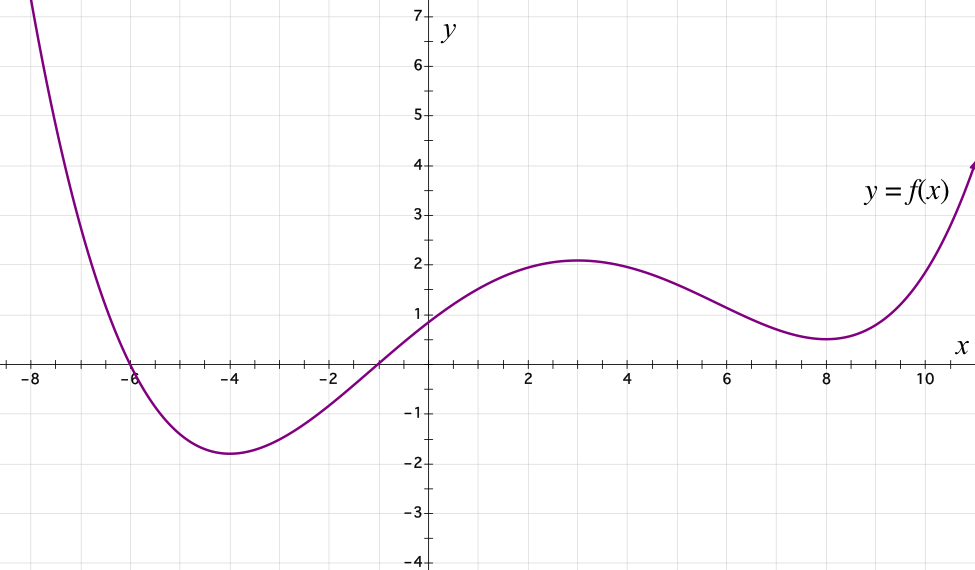
\includegraphics{Picture2.png}
\end{image}

\begin{problem}

For these questions, refer to the graph above.

\begin{enumerate}

\begin{tabular}{cc}

\begin{minipage}[t]{.5\textwidth}
\item On the interval $[-6, -4]$, is $f'(x)$:\hspace{1cm}\hspace{1cm}
\begin{itemize}
\item $<0$
\item $=0$
\item $>0$, or
\item more than one of the above
\end{itemize}
\end{minipage}

&

\begin{minipage}[t]{.5\textwidth}
\item On the interval $[-4, -2]$, is $f'(x)$:
\begin{itemize}
\item $<0$
\item $=0$
\item $>0$, or
\item more than one of the above
\end{itemize}
\end{minipage}

\\

\begin{minipage}[t]{.5\textwidth}
\item On the interval $[0, 2]$, is $f'(x)$:
\begin{itemize}
\item $<0$
\item $=0$
\item $>0$, or
\item more than one of the above
\end{itemize}
\end{minipage}

&

\begin{minipage}[t]{.5\textwidth}
\item On the interval $[2, 4]$, is $f'(x)$:
\begin{itemize}
\item $<0$
\item $=0$
\item $>0$, or
\item more than one of the above
\end{itemize}
\end{minipage}

\end{tabular}

\end{enumerate}

\end{problem}

\begin{problem}
For these questions, refer to the graph above.


\begin{enumerate}

\begin{tabular}{lr}


\begin{minipage}[t]{.5\textwidth}
\item On the interval $[-6, -4]$, is $f'(x)$:\hspace{1cm}\hspace{1cm}
\begin{itemize}
\item increasing
\item decreasing, or
\item more than one of the above
\end{itemize}
\end{minipage}

&

\begin{minipage}[t]{.5\textwidth}
\item On the interval $[-4, -2]$, is $f'(x)$:
\begin{itemize}
\item increasing
\item decreasing, or
\item more than one of the above
\end{itemize}
\end{minipage}

\\

\begin{minipage}[t]{.5\textwidth}
\item On the interval $[0, 2]$, is $f'(x)$:
\begin{itemize}
\item increasing
\item decreasing, or
\item more than one of the above
\end{itemize}
\end{minipage}

&

\begin{minipage}[t]{.5\textwidth}
\item On the interval $[2, 4]$, is $f'(x)$:
\begin{itemize}
\item increasing
\item decreasing, or
\item more than one of the above
\end{itemize}
\end{minipage}

\end{tabular}

\end{enumerate}

\end{problem}

\begin{problem}
For how many values of $x$ in the interval $[-8, 10]$ does $f'(x)=0$?
\end{problem}

\begin{problem}
From following expressions, identify the smallest and largest according to the numerical value they represent:

\begin{itemize}
\item $f'(8)$
\item $\dfrac{f(8+\Delta x)-f(8)}{\Delta x}$ for $\Delta x > 0$
\item $f(-6)$
\item $f'(-6)$
\end{itemize}
\end{problem}

\end{document}




